% Beamer presentation — 15 minutes
% Convergence of Policy Gradient Methods to Nash Equilibria in Stochastic Games
\documentclass[aspectratio=169,11pt]{beamer}

\usetheme{Madrid}
\usecolortheme{default}
\setbeamertemplate{navigation symbols}{}
\setbeamertemplate{footline}[frame number]

\usepackage{amsmath,amssymb,amsthm}
\usepackage{mathtools}
\usepackage{graphicx}
\usepackage{booktabs}
\usepackage{tikz}
\usetikzlibrary{positioning,arrows.meta}

% Commands
\newcommand{\calS}{\mathcal{S}}
\newcommand{\calA}{\mathcal{A}}
\newcommand{\calN}{\mathcal{N}}
\newcommand{\calG}{\mathcal{G}}
\newcommand{\calU}{\mathcal{U}}
\newcommand{\ip}[2]{\langle #1,\, #2 \rangle}
\newcommand{\norm}[1]{\| #1 \|}
\newcommand{\R}{\mathbb{R}}
\newcommand{\E}{\mathbb{E}}
\newcommand{\Prob}{\mathbb{P}}
\DeclareMathOperator*{\argmax}{arg\,max}
\DeclareMathOperator{\proj}{proj}

\title{Convergence of Policy Gradient Methods\\
  to Nash Equilibria in Stochastic Games}
\author{Yevhen Shcherbinin\\[4pt]
  {\small Candidate No.\ 60103}}
\institute{Department of Mathematics\\
  London School of Economics}
\date{2026}

\begin{document}

% ──────────────────────────────────────────────────────────
\begin{frame}
  \titlepage
\end{frame}

% ══════════════════════════════════════════════════════════
\section{Motivation}
% ══════════════════════════════════════════════════════════

\begin{frame}{Why Does This Matter?}
  \textbf{Algorithmic pricing is everywhere.}\\[4pt]
  Airlines, ride-sharing, e-commerce: prices are set by AI, in real time,
  millions of times a day.

  \bigskip

  These algorithms are not isolated --- they \textbf{interact}.
  Each one watches the others and adapts. They are, effectively, playing a game.

  \bigskip

  \textbf{The concern regulators have:}
  \begin{itemize}
    \item Can these algorithms learn to sustain artificially high prices\ldots
    \item \ldots\emph{without anyone programming them to collude?}
  \end{itemize}

  \bigskip

  Answering this rigorously requires understanding whether competitive
  learning processes \textbf{converge to a Nash equilibrium} ---
  and \textbf{this is exactly what this dissertation proves}.
\end{frame}

% ──────────────────────────────────────────────────────────
\begin{frame}{The Reinforcement Learning Loop}
  \begin{columns}[c]
    \begin{column}{0.42\textwidth}
      An agent interacts with an environment step by step:
      \begin{enumerate}
        \item Observe current \textbf{state} $s_t$
        \item Choose \textbf{action} $a_t$ via policy $\pi$
        \item Receive \textbf{reward} $r_t = R(s_t, a_t)$
        \item Environment moves to new state
      \end{enumerate}

      \bigskip

      \textbf{Markov property:} the next state depends only on
      $(s_t, a_t)$, not on the full history.
      \[
        s_{t+1} \sim \mathcal{P}(\,\cdot \mid s_t,\, a_t\,)
      \]

      \textbf{Goal:} find $\pi$ maximising
      $V^\pi = \E\bigl[\sum_t r_t\bigr]$.
    \end{column}
    \begin{column}{0.55\textwidth}
      \centering
      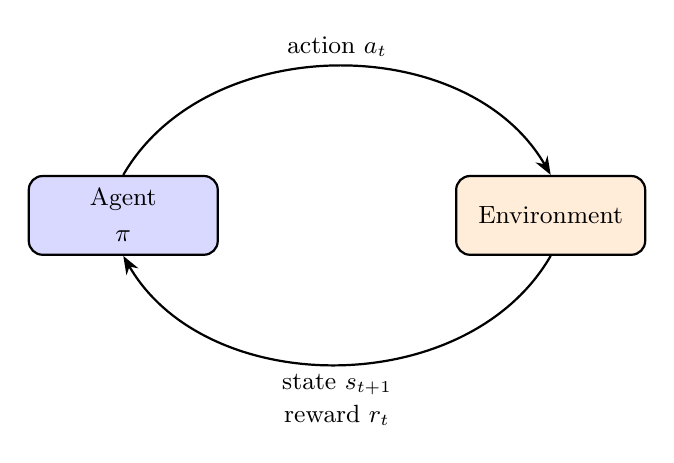
\begin{tikzpicture}[
          >=Stealth, thick,
          box/.style={draw, rounded corners=5pt,
                      minimum width=2.4cm, minimum height=1cm,
                      align=center, font=\small}
        ]
        \node[box, fill=blue!15]   (agent) {Agent\\[2pt]$\pi$};
        \node[box, fill=orange!15, right=3cm of agent] (env)
              {Environment};

        % action arrow
        \draw[->] (agent.north) to[out=60,in=120]
          node[above]{\small action $a_t$}
          (env.north);

        % state + reward arrow
        \draw[->] (env.south) to[out=240,in=300]
          node[below, align=center]
            {\small state $s_{t+1}$\\\small reward $r_t$}
          (agent.south);
      \end{tikzpicture}

      \vspace{0.4cm}
      {\small (This is a \textbf{Markov Decision Process}.\\
      Stochastic games generalise it to $N$ agents.)}
    \end{column}
  \end{columns}
\end{frame}

% ──────────────────────────────────────────────────────────
\begin{frame}{What is Known (and What Isn't)}
  \begin{columns}[c]
    \begin{column}{0.45\textwidth}
      \textbf{Solved in special cases:}
      \begin{itemize}
        \item All players share the same goal \\ {\small(potential games)}
        \item Two players, strictly opposed \\ {\small(zero-sum games, under extra conditions)}
      \end{itemize}
      \medskip
      Convergence guarantees exist in these cases.
    \end{column}
    \begin{column}{0.45\textwidth}
      \textbf{Open --- the general case:}
      \begin{itemize}
        \item Mixed motives (partly competing, partly cooperating)
        \item Many players
        \item The environment has multiple states
      \end{itemize}
      \medskip
      No convergence guarantee existed for this setting.
    \end{column}
  \end{columns}

  \bigskip

  \begin{center}
    \textbf{This dissertation:} prove convergence in the general case,\\
    and make it \emph{global} (independent of where you start).
  \end{center}
\end{frame}

% ──────────────────────────────────────────────────────────
\begin{frame}{Stochastic Games: $N$ Agents in a Shared MDP}
  Replace the single agent with $N$ agents, all learning at once.

  \medskip

  \[
    \mathcal{G} = \langle\;
      \underbrace{\mathcal{N}}_{\text{players}},\quad
      \underbrace{\mathcal{S}}_{\text{states}},\quad
      \underbrace{(\mathcal{A}_i)}_{\text{actions}},\quad
      \underbrace{(R_i)}_{\text{rewards}},\quad
      \underbrace{\mathcal{P}}_{\text{transitions}},\quad
      \underbrace{\rho}_{\text{start}}
    \;\rangle
  \]

  \smallskip

  \begin{tabular}{@{}lll@{}}
    $\mathcal{N} = \{1,\ldots,N\}$ & players \\[4pt]
    $\mathcal{S}$ & shared state space
      & {\small e.g.\ price levels, board position} \\[4pt]
    $\mathcal{A}_i$ & actions for player $i$
      & {\small joint action $a = (a_1,\ldots,a_N)$} \\[4pt]
    $R_i(s,a)\in\R$ & reward to player $i$
      & {\small each player has their \emph{own}} \\[4pt]
    $\mathcal{P}(s'\!\mid\!s,a)$ & transition kernel
      & {\small same Markov dynamics as before} \\[4pt]
    $\rho$ & initial state distribution \\
  \end{tabular}

  \smallskip

  \textbf{Policy} $\pi_i(a\mid s)$: probability of action $a$ in state $s$.\quad
  \textbf{Value:} $V_i(\pi) = \E\bigl[\sum_t R_i(s_t,a_t)\bigr]$.

  \textbf{Nash equilibrium} $\pi^*$: no player gains by deviating unilaterally.\\
  {\small\textit{Think: a stable resting point — everyone plays their best response to everyone else.}}
\end{frame}

% ══════════════════════════════════════════════════════════
\section{Local Convergence (Chapter 3)}
% ══════════════════════════════════════════════════════════

\begin{frame}{Policy Gradient: The Update Rule}
  Each agent does gradient ascent on its own value, projected onto the strategy space:
  \[
    \pi_{n+1} = \proj_\Pi\!\bigl(\pi_n + \gamma_n\,\hat v_n\bigr)
  \]

  \begin{itemize}
    \item $\hat v_n \approx \nabla_{\pi_i} V_i(\pi_n)$ for each agent $i$ \quad --- estimated from sampled trajectories (REINFORCE)
    \item $\gamma_n \to 0$ \quad --- decaying step size
  \end{itemize}

  \bigskip\bigskip

  \begin{block}{Theorem 3.1 (Local Convergence)}
    If $\pi_0$ starts close enough to a \emph{stable} Nash equilibrium $\pi^*$
    {\normalfont\small(stable = small deviations self-correct)},
    \[
      \Prob\!\bigl(\pi_n \to \pi^* \text{ as } n\to\infty\bigr) = 1
    \]
  \end{block}
\end{frame}

% ──────────────────────────────────────────────────────────
\begin{frame}{Why It Converges: The Lyapunov Argument}
  Define the \textbf{energy} $E_n = \norm{\pi_n - \pi^*}^2$ \quad (squared distance to Nash).

  \bigskip

  The update rule gives:
  \[
    E_{n+1} \;\le\; E_n
    \underbrace{-\, 2\gamma_n \ip{v(\pi_n)}{\pi_n - \pi^*}}_{\text{always negative near } \pi^*}
    +\; \underbrace{\text{noise} + \text{bias}}_{\text{controlled}}
  \]

  \bigskip

  Energy \emph{tends to decrease} --- with controlled random fluctuations.\\[6pt]
  A classical lemma (Robbins--Siegmund) turns this into almost-sure convergence.

  \bigskip

  \textbf{Our contribution:} a fully rigorous, self-contained version of this argument ---\\
  every probability space and random variable verified explicitly.
\end{frame}

% ══════════════════════════════════════════════════════════
\section{Global Convergence via Restarts (Chapter 4)}
% ══════════════════════════════════════════════════════════

\begin{frame}{The Initialisation Problem}
  Local convergence only kicks in if you \emph{start close enough} to Nash.\\
  In practice, agents have no idea where Nash equilibria are.

  \bigskip

  \textbf{Solution:} \emph{Random restarts.}

  \begin{block}{Algorithm: Restart-PG}
    \begin{enumerate}
      \item Pick a random starting strategy $\pi_0^{(k)}$ uniformly
      \item Run gradient ascent for $T$ steps $\to$ candidate $\hat\pi^{(k)}$
      \item If converged: stop.\quad Else: $k \gets k+1$, go to 1.
    \end{enumerate}
  \end{block}

  \bigskip

  \textbf{Key quantity:} the \emph{basin probability} $p$ = fraction of the
  strategy space that flows toward \emph{some} Nash equilibrium under
  gradient ascent. \quad As long as $p > 0$, restarts eventually succeed.
\end{frame}

% ──────────────────────────────────────────────────────────
\begin{frame}{Main Result: Almost-Sure Convergence}
  \begin{block}{Theorem 4.2 (Original Contribution)}
    Under mild regularity conditions, Restart-PG converges to a Nash
    equilibrium \textbf{almost surely} (= with probability 1):
    \[
      \Prob\bigl(K^* < \infty\bigr) = 1
    \]
    with geometric tail:\quad
    $\Prob(K^* > k) \le (1 - p)^k$
  \end{block}

  \begin{itemize}
    \item $K^*$ = number of restarts until convergence;\quad
          $\E[K^*] \le 1/p$
    \item \textbf{Equilibrium selection:} running $K$ restarts and
      keeping the best outcome approaches the \textbf{Pareto optimum}
      --- the outcome where no one can be made better off
      without making someone else worse off
  \end{itemize}
\end{frame}

% ──────────────────────────────────────────────────────────
\begin{frame}{Blessing of Dimensionality}
  \textbf{Worry:} Basin volume shrinks exponentially in dimension
  $d = \dim(\Pi)$.

  \bigskip

  \textbf{Key insight:} When Nash strategies are \emph{sparse} (only
  $k$ actions matter, $k \ll d$):
  \begin{itemize}
    \item The attraction basins extend broadly in the $d - k$
      ``irrelevant'' directions --- they are large in practice
    \item Empirically observed restart cost:
      $\mathcal{O}(k \log d)$ instead of $\mathcal{O}(d)$
    \item Confirmed empirically: a single restart sufficed ($K^* = 1$)
      for all tested games up to $d = 7$ strategy dimensions
  \end{itemize}

  \bigskip

  \textbf{Implication:} Restarts are practical, not just
  theoretical.
\end{frame}

% ══════════════════════════════════════════════════════════
\section{Empirical Validation}
% ══════════════════════════════════════════════════════════

\begin{frame}{Single-State Games: Basins and Equilibrium Selection}
  \begin{columns}[T]
    \begin{column}{0.48\textwidth}
      \textbf{Basins of attraction}\\[4pt]
      \includegraphics[width=\textwidth]{simulations/figures/restart_pg/basins_of_attraction.pdf}\\[2pt]
      {\small Coloured regions = which Nash equilibrium you land on
        from each starting point. They tile the whole space: a single
        random restart almost always suffices ($p \approx 1$).}
    \end{column}
    \begin{column}{0.48\textwidth}
      \textbf{Equilibrium selection}\\[4pt]
      
\includegraphics[width=\textwidth]{simulations/figures/restart_pg/equilibrium_selection.pdf}\\[2pt]
      {\small \textbf{Stag Hunt}: 2 hunters. Both cooperate $\to$ stag (best).
        One defects $\to$ defector gets rabbit, cooperator gets nothing.
        Best-of-$K$ restarts reliably finds the cooperative equilibrium.}
    \end{column}
  \end{columns}
\end{frame}

% ──────────────────────────────────────────────────────────
\begin{frame}{Two-State Game: Key Findings}
  \begin{columns}[T]
    \begin{column}{0.48\textwidth}
      \textbf{State structure matters}\\[4pt]
      \includegraphics[width=\textwidth]{simulations/figures/stochastic_pg/stochastic_vs_normal.pdf}\\[2pt]
      {\small Agents using state: SW $= 5.0$.\\
      Agents ignoring state: SW $\approx 3.1$.\\
      \textbf{38\% welfare gap} from collapsing the state space.}
    \end{column}
    \begin{column}{0.48\textwidth}
      \textbf{Restarts select the best equilibrium}\\[4pt]
      \includegraphics[width=\textwidth]{simulations/figures/stochastic_pg/stochastic_restarts.pdf}\\[2pt]
      {\small Single restarts land on different Nash equilibria.\\
      Best-of-$K$ reliably finds the Pareto-optimal outcome.}
    \end{column}
  \end{columns}
\end{frame}

% ══════════════════════════════════════════════════════════
\section{Contributions \& Future Work}
% ══════════════════════════════════════════════════════════

\begin{frame}{Summary of Contributions}
  \begin{enumerate}
    \item \textbf{Expository:} A fully rigorous, self-contained proof
      of gradient learning convergence to Nash in general multi-state
      games (Chapters 2--3)

      \medskip

    \item \textbf{Original:} Global convergence via restarts
      (Theorem 4.2) --- removes dependence on initialisation

      \medskip

    \item \textbf{Empirical:} Validation on normal-form and
      stochastic games, demonstrating:
      \begin{itemize}
        \item Basin probability $p \approx 1$ --- one restart
          almost always suffices in practice
        \item Best-of-$K$ restarts reliably selects the
          Pareto-optimal (best joint) equilibrium
        \item Ignoring state structure costs 38\% of achievable
          social welfare in the 2-state game
      \end{itemize}
  \end{enumerate}
\end{frame}

% ──────────────────────────────────────────────────────────
\begin{frame}{Where Next?}
  \begin{columns}[T]
    \begin{column}{0.55\textwidth}
      \textbf{The most compelling open direction:}

      \bigskip

      \textbf{Meta-learning} --- agents that don't just respond
      to opponents, but \emph{anticipate} how opponents will learn
      and actively steer their updates.

      \bigskip

      This is the mechanism behind \textbf{algorithmic collusion}:
      an agent that teaches its competitor to cooperate by shaping
      how the competitor's gradient updates unfold.

      \bigskip

      {\small This dissertation provides the convergence foundation
      that makes such analysis rigorous.}
    \end{column}
    \begin{column}{0.4\textwidth}
      \textbf{Other directions:}
      \begin{itemize}
        \item Neural network policies
        \item Sample complexity bounds
        \item Smarter restart strategies
        \item Continuous action spaces
      \end{itemize}
    \end{column}
  \end{columns}

  \medskip

  \begin{center}
    \emph{Local convergence $+$ random restarts $=$ global convergence.\\
    Simple, provably correct, empirically effective.}
  \end{center}
\end{frame}

% ──────────────────────────────────────────────────────────
\begin{frame}{Thank You}
  \begin{center}
    {\Large Thank you for your attention.}

    \bigskip\bigskip

    {\large Yevhen Shcherbinin}\\[4pt]
    Candidate No.\ 60103\\[4pt]
    Department of Mathematics, LSE

    \bigskip\bigskip

    {\small Supervised by Prof.\ Galit Ashkenazi-Golan}
  \end{center}
\end{frame}

% ──────────────────────────────────────────────────────────
\begin{frame}[allowframebreaks]{References}
  \small
  \nocite{giannou2022,kalogiannis2025,leung2024,anagnostides2024,foster2023,kim2021}
  \bibliographystyle{plainnat}
  \bibliography{references}
\end{frame}

\end{document}
